\documentclass[10pt,a4paper]{article}
\usepackage[margin=18mm,top=20mm,bottom=18mm]{geometry}
\usepackage{fontspec,graphicx,amsmath,booktabs,xcolor,fancyhdr}
\setmainfont{DejaVu Sans}
\newfontfamily\jpfont[Path=/usr/share/fonts/google-droid-sans-fonts/,BoldFont=DroidSansFallbackFull.ttf,BoldFeatures={FakeBold=1.2}]{DroidSansFallbackFull.ttf}
\XeTeXlinebreaklocale "ja"
\XeTeXlinebreakskip=0pt plus 1pt
\definecolor{navy}{HTML}{17385D}
\pagestyle{fancy}\fancyhf{}\fancyhead[L]{\small STAR / Nuclear PID and Purity}\fancyhead[R]{\small He4 / region-specific models}\fancyfoot[C]{\thepage}\setlength{\headheight}{14pt}
\emergencystretch=2em\setlength{\parindent}{0pt}\setlength{\parskip}{5pt}\linespread{1.10}
\begin{document}
\section*{⁴He\hspace{0pt}{\jpfont の}\hspace{0pt}PID\hspace{0pt}{\jpfont 係数更新と}\hspace{0pt}Purity\hspace{0pt}{\jpfont 推定}\hspace{0pt}}
2026\hspace{0pt}{\jpfont 年}\hspace{0pt}10\hspace{0pt}{\jpfont 月}\hspace{0pt}22\hspace{0pt}{\jpfont 日}\hspace{0pt} /\allowbreak{} 2021 P24iy\hspace{0pt}{\jpfont 、}\hspace{0pt}auau3p85\hspace{0pt}{\jpfont 解析試料}\hspace{0pt}

\hspace{0pt}{\jpfont 既存の}\hspace{0pt}2021 P24iy\hspace{0pt}{\jpfont 部分統合試料を使い、対象を}\hspace{0pt}⁴He\hspace{0pt}{\jpfont だけに絞る。}\hspace{0pt}d\hspace{0pt}{\jpfont 、}\hspace{0pt}t\hspace{0pt}{\jpfont 、}\hspace{0pt}³He\hspace{0pt}{\jpfont の}\hspace{0pt}PID\hspace{0pt}{\jpfont 関数形・係数・元の適用域は}\hspace{0pt}Git 8f7d539\hspace{0pt}{\jpfont に固定し、}\hspace{0pt}⁴He\hspace{0pt}{\jpfont だけ従来多項式の係数を調整した。低}\hspace{0pt}R\hspace{0pt}{\jpfont と}\hspace{0pt}TOF\hspace{0pt}{\jpfont 領域を指定の異なるモデルで評価する。}\hspace{0pt}

\begin{center}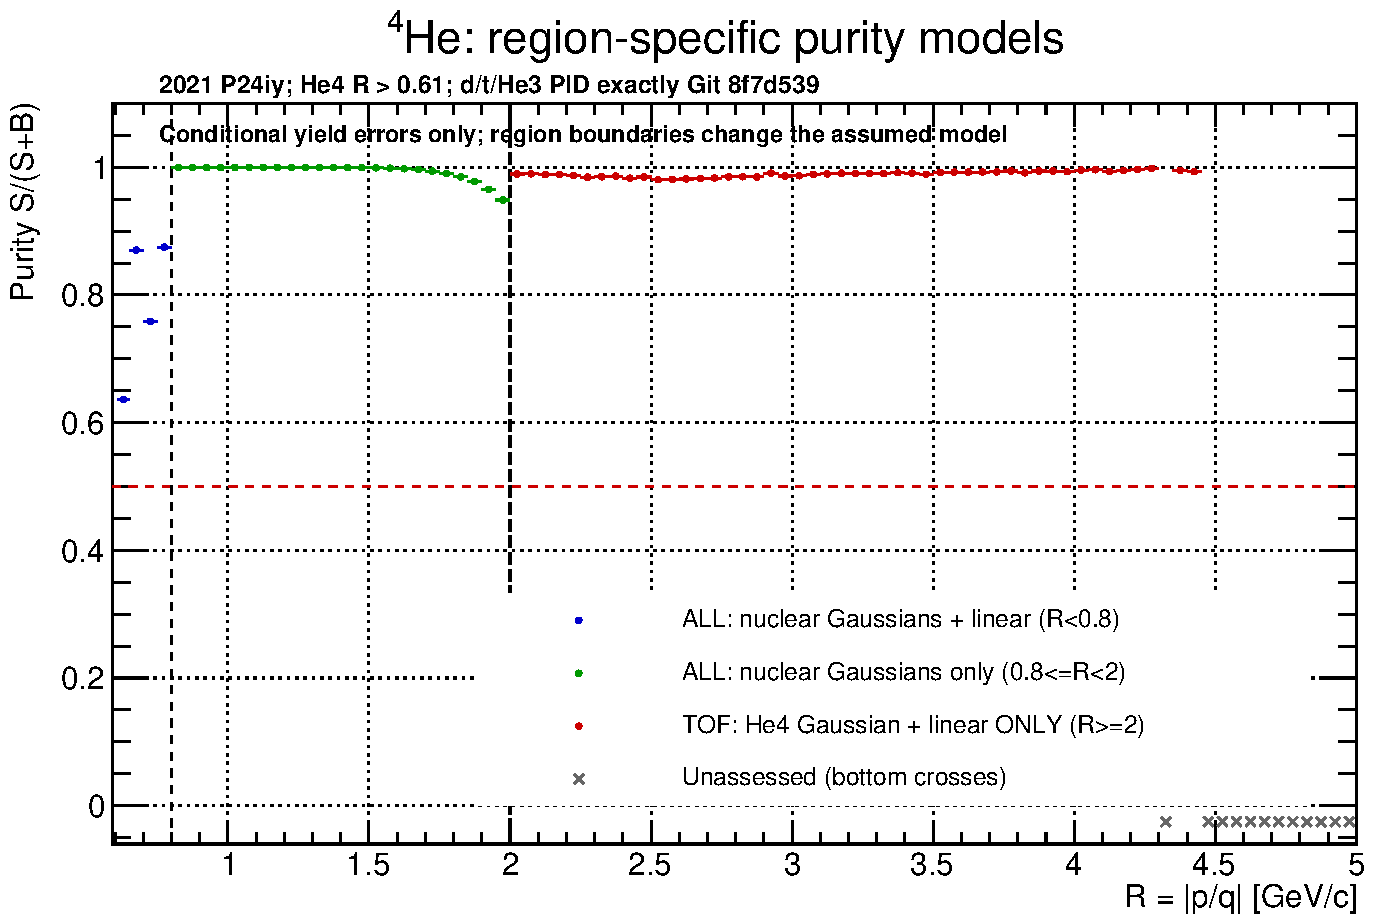
\includegraphics[width=\linewidth,height=.56\textheight,keepaspectratio]{purity_vs_p_over_q_01_trim.png}\end{center}
\hspace{0pt}{\jpfont 図}\hspace{0pt}1\hspace{0pt}{\jpfont 　}\hspace{0pt}⁴He\hspace{0pt}{\jpfont の最終}\hspace{0pt}Purity\hspace{0pt}{\jpfont 。青：}\hspace{0pt}ALL\hspace{0pt}{\jpfont の}\hspace{0pt}Gaussian\hspace{0pt}{\jpfont ＋}\hspace{0pt}linear\hspace{0pt}{\jpfont 、緑：}\hspace{0pt}ALL\hspace{0pt}{\jpfont の}\hspace{0pt}Gaussian\hspace{0pt}{\jpfont のみ、赤：}\hspace{0pt}TOF\hspace{0pt}{\jpfont の}\hspace{0pt}⁴He Gaussian\hspace{0pt}{\jpfont ＋}\hspace{0pt}linear\hspace{0pt}{\jpfont のみ。灰色}\hspace{0pt}×\hspace{0pt}{\jpfont は未支持区間の位置を下端へ示し、}\hspace{0pt}Purity=0\hspace{0pt}{\jpfont を意味しない。境界でモデルと試料が変わるため、点を線で接続していない。}\hspace{0pt}

R=0.61–0.65\hspace{0pt}{\jpfont の}\hspace{0pt}Purity\hspace{0pt}{\jpfont は}\hspace{0pt}63.66 ± 0.07\%\hspace{0pt}{\jpfont （条件付き収量誤差）。全}\hspace{0pt}88\hspace{0pt}{\jpfont 集約区間中}\hspace{0pt}76\hspace{0pt}{\jpfont 区間が支持条件を通過。本番設定への反映は行っていない。}\hspace{0pt}


\clearpage
\section*{1. \hspace{0pt}{\jpfont 選択と}\hspace{0pt}3\hspace{0pt}{\jpfont 領域の評価モデル}\hspace{0pt}}
\begin{center}\small\begin{tabular}{lrr}\toprule
R [GeV/\allowbreak{}c] & \hspace{0pt}{\jpfont 試料}\hspace{0pt} & fit\hspace{0pt}{\jpfont の成分}\hspace{0pt}\\\midrule
{}0.61–0.80 & ALL\hspace{0pt}{\jpfont 、}\hspace{0pt}TOF\hspace{0pt}{\jpfont なし}\hspace{0pt} & d/\allowbreak{}t/\allowbreak{}³He/\allowbreak{}⁴He Gaussian\hspace{0pt}{\jpfont ＋}\hspace{0pt}linear\\
{}0.80–2.00 & ALL\hspace{0pt}{\jpfont 、}\hspace{0pt}TOF\hspace{0pt}{\jpfont なし}\hspace{0pt} & d/\allowbreak{}t/\allowbreak{}³He/\allowbreak{}⁴He Gaussian\hspace{0pt}{\jpfont のみ}\hspace{0pt}\\
{}2.00–5.00 & \hspace{0pt}{\jpfont 既存}\hspace{0pt}TAG\_\allowbreak{}D & ⁴He Gaussian\hspace{0pt}{\jpfont ＋}\hspace{0pt}linear\hspace{0pt}{\jpfont のみ}\hspace{0pt}\\\bottomrule\end{tabular}\end{center}
R=|p/\allowbreak{}q|\hspace{0pt}{\jpfont 。}\hspace{0pt}⁴He\hspace{0pt}{\jpfont は}\hspace{0pt}strict R>0.61\hspace{0pt}{\jpfont 、}\hspace{0pt}0.80\hspace{0pt}{\jpfont は背景なし側に含める。}\hspace{0pt}TOF\hspace{0pt}{\jpfont 側は}\hspace{0pt}R=2.00\hspace{0pt}{\jpfont からの}\hspace{0pt}native\hspace{0pt}{\jpfont 区間を使う。境界点}\hspace{0pt}R=2\hspace{0pt}{\jpfont 自体は連続分布上で測度}\hspace{0pt}0\hspace{0pt}{\jpfont であり、区間に重複・欠落はない。}\hspace{0pt}⁴He\hspace{0pt}{\jpfont の}\hspace{0pt}TOF m²\hspace{0pt}{\jpfont 窓は}\hspace{0pt}d\hspace{0pt}{\jpfont と同一の}\hspace{0pt}strict 3.268773<m²<3.693147\hspace{0pt}{\jpfont 。}\hspace{0pt}

TPC\hspace{0pt}{\jpfont 選択は全}\hspace{0pt}4\hspace{0pt}{\jpfont 核種の}\hspace{0pt}|nσ|<2\hspace{0pt}{\jpfont と}\hspace{0pt}best-species\hspace{0pt}{\jpfont 判定。競合時は}\hspace{0pt}|nσ|\hspace{0pt}{\jpfont 最小、同値の優先順}\hspace{0pt}d\hspace{0pt}{\jpfont 、}\hspace{0pt}t\hspace{0pt}{\jpfont 、}\hspace{0pt}³He\hspace{0pt}{\jpfont 、}\hspace{0pt}⁴He\hspace{0pt}{\jpfont 。}\hspace{0pt}d/\allowbreak{}t/\allowbreak{}³He\hspace{0pt}{\jpfont 自身の式が固定でも、}\hspace{0pt}⁴He\hspace{0pt}{\jpfont の係数変更により競合境界は変わるため、新しい全核種の選択窓を使って積分し直した。}\hspace{0pt}

\[n\sigma_i=\frac{dE/dx-\mu_{{\rm PID},i}(R)}{\sigma_{{\rm PID},i}(R)},\qquad P_4=\frac{S_4}{S_4+B}.\]
\hspace{0pt}{\jpfont 低}\hspace{0pt}R\hspace{0pt}{\jpfont の}\hspace{0pt}B\hspace{0pt}{\jpfont は選択窓に入る他核種と、背景あり領域では}\hspace{0pt}linear\hspace{0pt}{\jpfont の寄与。高}\hspace{0pt}R\hspace{0pt}{\jpfont の}\hspace{0pt}B\hspace{0pt}{\jpfont は}\hspace{0pt}linear\hspace{0pt}{\jpfont だけであり、他核種の}\hspace{0pt}Gaussian\hspace{0pt}{\jpfont 成分は}\hspace{0pt}fit\hspace{0pt}{\jpfont にも分母にも入れない。これはユーザー指定モデルの仮定であり、データから他核種が不存在と証明したものではない。}\hspace{0pt}

\[\text{TOF:}\quad f=N_4G_4+B_{\rm linear},\qquad P_4=\frac{\int_{\rm PID}N_4G_4}{\int_{\rm PID}(N_4G_4+B_{\rm linear})}.\]
\hspace{0pt}{\jpfont 低}\hspace{0pt}R native\hspace{0pt}{\jpfont 幅}\hspace{0pt}0.01\hspace{0pt}{\jpfont 、}\hspace{0pt}TOF\hspace{0pt}{\jpfont 側は既存}\hspace{0pt}0.05 GeV/\allowbreak{}c\hspace{0pt}{\jpfont 。}\hspace{0pt}Purity\hspace{0pt}{\jpfont 表示は}\hspace{0pt}0.05\hspace{0pt}{\jpfont 幅へ}\hspace{0pt}ΣS/\allowbreak{}Σtotal\hspace{0pt}{\jpfont で集約し、最初のみ}\hspace{0pt}0.61–0.65\hspace{0pt}{\jpfont へ}\hspace{0pt}clip\hspace{0pt}{\jpfont する。}\hspace{0pt}R\hspace{0pt}{\jpfont 方向は}\hspace{0pt}GL3\hspace{0pt}{\jpfont で積分、生計数は}\hspace{0pt}native dE/\allowbreak{}dx bin\hspace{0pt}{\jpfont の重なり比から独立計数する。}\hspace{0pt}


\clearpage
\section*{2. Git\hspace{0pt}{\jpfont 固定値と}\hspace{0pt}⁴He\hspace{0pt}{\jpfont 候補の係数}\hspace{0pt}}
\[x=\log_{10}(R/(1\,{\rm GeV}/c)),\quad\mu_{\rm PID}=a_0+a_1x+a_2x^2+a_3x^3,\quad\sigma_{\rm PID}=b_0+b_1x+b_2x^2.\]
\begin{center}\small\begin{tabular}{lrrrr}\toprule
\hspace{0pt}{\jpfont 核種}\hspace{0pt} & a0 & a1 & a2 & a3\\\midrule
{}d\hspace{0pt}{\jpfont ・固定}\hspace{0pt} & 10.2875 & -36.6639 & 67.63 & -45.2483\\
{}t\hspace{0pt}{\jpfont ・固定}\hspace{0pt} & 19.2177 & -70.3198 & 113.876 & -67.0591\\
{}³He\hspace{0pt}{\jpfont ・固定}\hspace{0pt} & 28.8747 & -68.8637 & 104.455 & -56.9342\\
{}⁴He\hspace{0pt}{\jpfont ・元}\hspace{0pt} & 39.974 & -103.365 & 139.182 & -67.1446\\
{}⁴He\hspace{0pt}{\jpfont ・候補}\hspace{0pt} & 40.0707543 & -104.698411 & 140.399578 & -64.6344839\\\bottomrule\end{tabular}\end{center}
\begin{center}\small\begin{tabular}{lrrr}\toprule
\hspace{0pt}{\jpfont 核種}\hspace{0pt} & b0 & b1 & b2\\\midrule
{}d\hspace{0pt}{\jpfont ・固定}\hspace{0pt} & 0.771189 & -2.63609 & 2.8044\\
{}t\hspace{0pt}{\jpfont ・固定}\hspace{0pt} & 1.40996 & -4.97147 & 4.97608\\
{}³He\hspace{0pt}{\jpfont ・固定}\hspace{0pt} & 1.636 & -4.35588 & 4.40594\\
{}⁴He\hspace{0pt}{\jpfont ・元}\hspace{0pt} & 2.24127 & -7.08328 & 8.07124\\
{}⁴He\hspace{0pt}{\jpfont ・候補}\hspace{0pt} & 2.36880488 & -6.95722547 & 7.1248802\\\bottomrule\end{tabular}\end{center}
Git\hspace{0pt}{\jpfont ヘッダを直接保存し、}\hspace{0pt}d/\allowbreak{}t/\allowbreak{}³He\hspace{0pt}{\jpfont の係数・関数形・適用域の一致を検証した。以前の}\hspace{0pt}study\hspace{0pt}{\jpfont で微調整した}\hspace{0pt}³He\hspace{0pt}{\jpfont 係数は使用していない。候補の全桁は}\hspace{0pt}coefficients.json\hspace{0pt}{\jpfont と}\hspace{0pt}candidate\_\allowbreak{}pid/\allowbreak{}NuclearIdDeDxVsMom.h\hspace{0pt}{\jpfont に保存し、}\hspace{0pt}Git\hspace{0pt}{\jpfont との差分も同梱する。}\hspace{0pt}

\hspace{0pt}{\jpfont 基準}\hspace{0pt}3\hspace{0pt}{\jpfont 領域}\hspace{0pt}fit\hspace{0pt}{\jpfont の}\hspace{0pt}199\hspace{0pt}{\jpfont 点中}\hspace{0pt}169\hspace{0pt}{\jpfont 点を、数値成立・形状支持・局所残差と}\hspace{0pt}R=0.61–3.5\hspace{0pt}{\jpfont で選んで係数を推定。元の}\hspace{0pt}σ\hspace{0pt}{\jpfont 単位で等しい重みの最小二乗を用い、}\hspace{0pt}Purity\hspace{0pt}{\jpfont 最大化による調整はしない。中心は元}\hspace{0pt}σ\hspace{0pt}{\jpfont の}\hspace{0pt}0.5\hspace{0pt}{\jpfont 倍、幅は元}\hspace{0pt}σ\hspace{0pt}{\jpfont の}\hspace{0pt}20\%\hspace{0pt}{\jpfont 以内へ変化を制限した。}\hspace{0pt}

\hspace{0pt}{\jpfont 監査域}\hspace{0pt}R=0.61–5\hspace{0pt}{\jpfont の}\hspace{0pt}1,001\hspace{0pt}{\jpfont 点で正の中心・幅と変更量を確認。中心の正規化}\hspace{0pt}RMS\hspace{0pt}{\jpfont は}\hspace{0pt}0.268→0.210\hspace{0pt}{\jpfont 、幅は}\hspace{0pt}0.218→0.146\hspace{0pt}{\jpfont 。}\hspace{0pt}PID\hspace{0pt}{\jpfont 関数とスペクトル応答の中心・幅は別の量である。}\hspace{0pt}


\clearpage
\section*{3. ⁠⁴He\hspace{0pt}{\jpfont の中心・幅の変更前後}\hspace{0pt}}
\begin{center}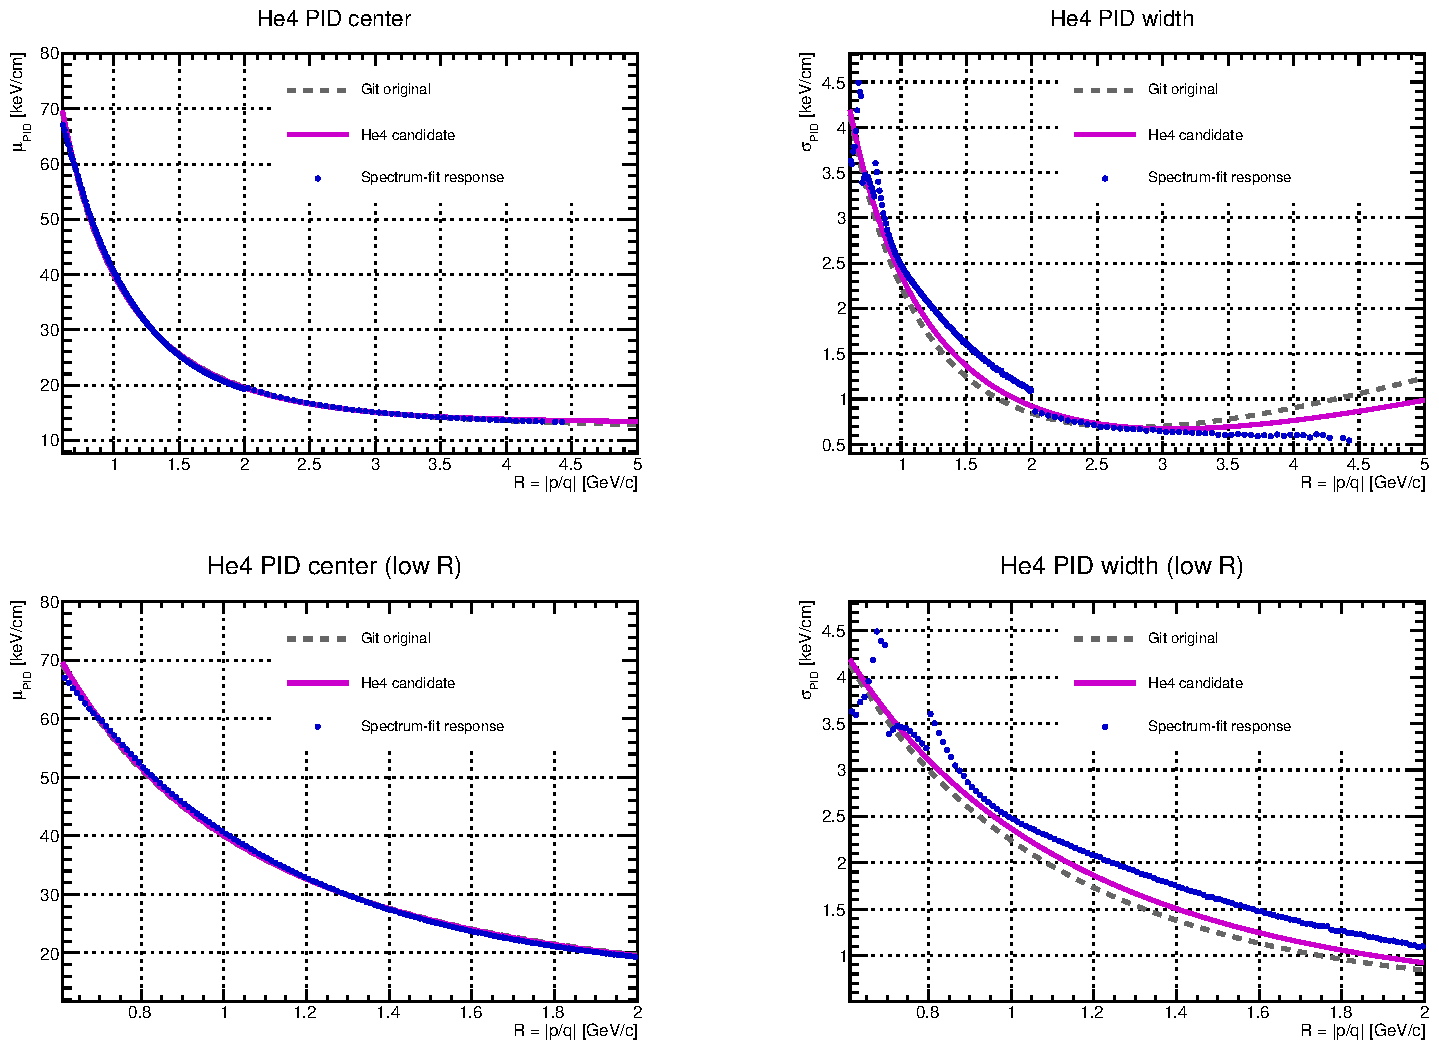
\includegraphics[width=\linewidth,height=.71\textheight,keepaspectratio]{pid_functions_01_trim.png}\end{center}
\hspace{0pt}{\jpfont 図}\hspace{0pt}2\hspace{0pt}{\jpfont 　灰色破線は}\hspace{0pt}Git\hspace{0pt}{\jpfont 元}\hspace{0pt}PID\hspace{0pt}{\jpfont 、紫は}\hspace{0pt}⁴He\hspace{0pt}{\jpfont 候補。上段は全}\hspace{0pt}R\hspace{0pt}{\jpfont 、下段は低}\hspace{0pt}R\hspace{0pt}{\jpfont 。青の点は支持された各スペクトル}\hspace{0pt}fit\hspace{0pt}{\jpfont の}\hspace{0pt}Gaussian\hspace{0pt}{\jpfont 応答で、}\hspace{0pt}PID\hspace{0pt}{\jpfont 選択窓の中心・幅と同一視しない。}\hspace{0pt}d/\allowbreak{}t/\allowbreak{}³He\hspace{0pt}{\jpfont は}\hspace{0pt}Git\hspace{0pt}{\jpfont 元係数のまま。}\hspace{0pt}

\hspace{0pt}{\jpfont 曲線は元の多項式で滑らかに定義し、}\hspace{0pt}R=0.8\hspace{0pt}{\jpfont や}\hspace{0pt}2.0\hspace{0pt}{\jpfont で}\hspace{0pt}PID\hspace{0pt}{\jpfont 関数を切り替えていない。境界で変わるのは}\hspace{0pt}Purity\hspace{0pt}{\jpfont の}\hspace{0pt}fit\hspace{0pt}{\jpfont モデルと}\hspace{0pt}TOF\hspace{0pt}{\jpfont 要求である。}\hspace{0pt}


\clearpage
\section*{4. ALL\hspace{0pt}{\jpfont 分布と}\hspace{0pt}PID\hspace{0pt}{\jpfont 選択曲線}\hspace{0pt}}
\begin{center}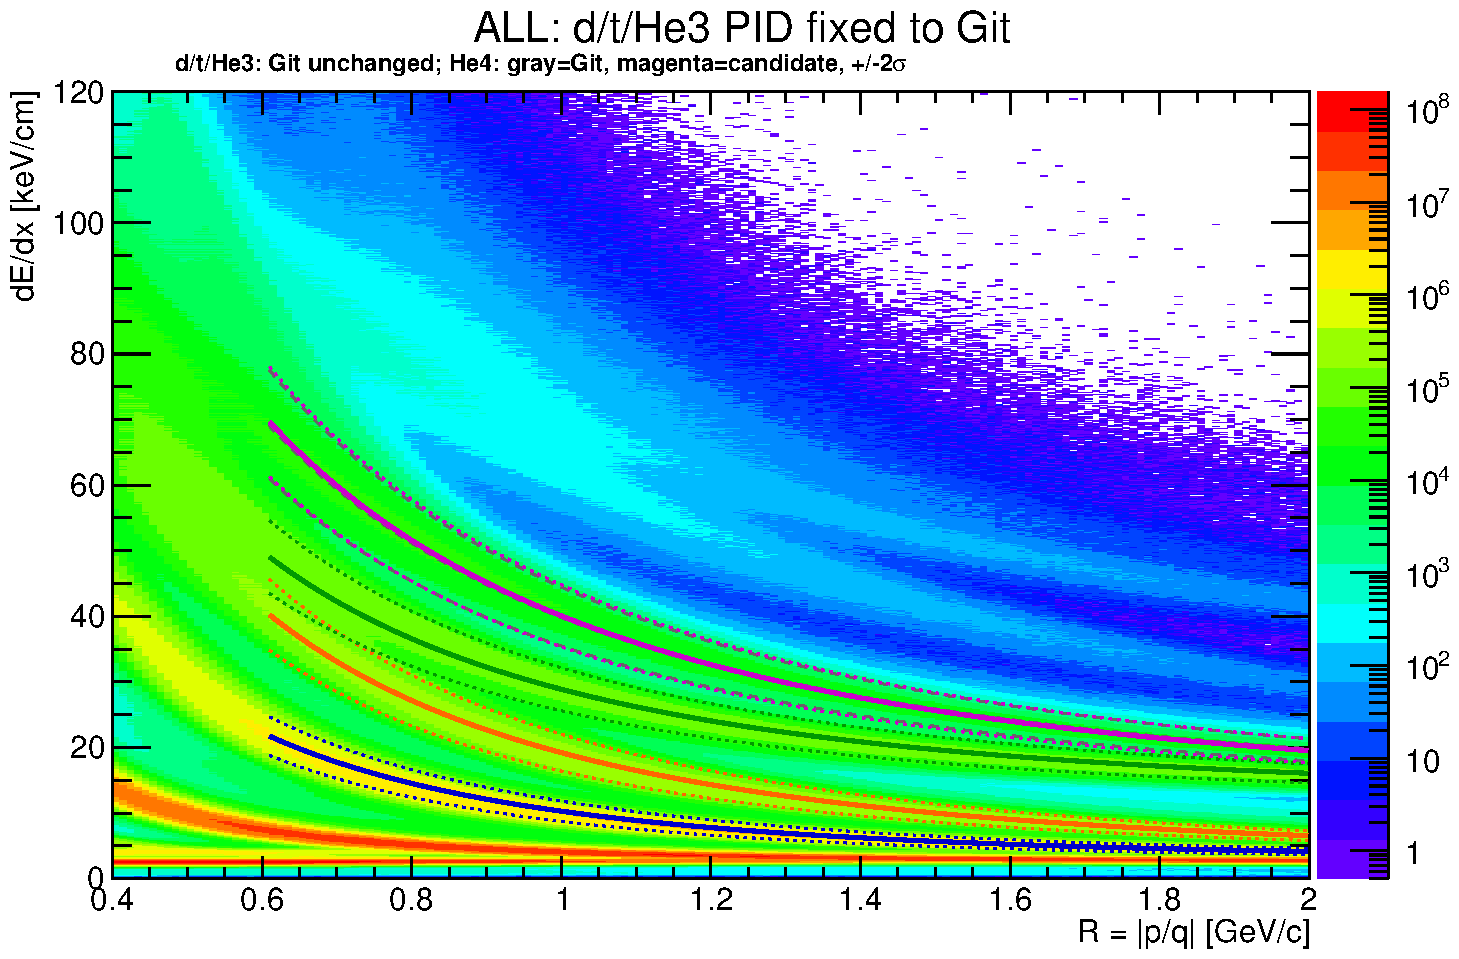
\includegraphics[width=\linewidth,height=.62\textheight,keepaspectratio]{dedx_pid_map_01_trim.png}\end{center}
\hspace{0pt}{\jpfont 図}\hspace{0pt}3\hspace{0pt}{\jpfont 　}\hspace{0pt}TOF\hspace{0pt}{\jpfont を要求しない}\hspace{0pt}ALL\hspace{0pt}{\jpfont の}\hspace{0pt}dE/\allowbreak{}dx\hspace{0pt}{\jpfont 対}\hspace{0pt}R\hspace{0pt}{\jpfont 。}\hspace{0pt}d/\allowbreak{}t/\allowbreak{}³He\hspace{0pt}{\jpfont は}\hspace{0pt}Git\hspace{0pt}{\jpfont 元の中心と}\hspace{0pt}±2σ\hspace{0pt}{\jpfont 、}\hspace{0pt}⁴He\hspace{0pt}{\jpfont は灰色の元関数と紫の候補を示す。実際の選択は帯の単独切出しに加え}\hspace{0pt}best-species\hspace{0pt}{\jpfont で区切る。}\hspace{0pt}

\hspace{0pt}{\jpfont 高}\hspace{0pt}R\hspace{0pt}{\jpfont で他核種の}\hspace{0pt}fit\hspace{0pt}{\jpfont 成分を除いたことは、}\hspace{0pt}TPC PID\hspace{0pt}{\jpfont の競合判定から}\hspace{0pt}d/\allowbreak{}t/\allowbreak{}³He\hspace{0pt}{\jpfont を取り除いたことを意味しない。元の競合判定を保った}\hspace{0pt}⁴He\hspace{0pt}{\jpfont 選択に対し、指定モデルで}\hspace{0pt}Purity\hspace{0pt}{\jpfont を求めた。}\hspace{0pt}

⁴He\hspace{0pt}{\jpfont の適用下限}\hspace{0pt}R>0.61\hspace{0pt}{\jpfont は}\hspace{0pt}pid\_\allowbreak{}selection.yaml\hspace{0pt}{\jpfont で明示する。候補ヘッダの元の関数適用域自体は保持しており、ヘッダだけで下限}\hspace{0pt}cut\hspace{0pt}{\jpfont まで実装したものではない。}\hspace{0pt}


\clearpage
\section*{5. \hspace{0pt}{\jpfont 代表}\hspace{0pt}fit\hspace{0pt}{\jpfont ：低}\hspace{0pt}R Gaussian\hspace{0pt}{\jpfont ＋}\hspace{0pt}linear}
R=[0.61,0.62)\hspace{0pt}{\jpfont 、}\hspace{0pt}[0.64,0.65)\hspace{0pt}{\jpfont 、}\hspace{0pt}[0.79,0.80) GeV/\allowbreak{}c\hspace{0pt}{\jpfont 。各段で左}\hspace{0pt}linear\hspace{0pt}{\jpfont 、右}\hspace{0pt}log\hspace{0pt}{\jpfont 表示。}\hspace{0pt}⁴He\hspace{0pt}{\jpfont の中心・幅は自由}\hspace{0pt}fit\hspace{0pt}{\jpfont 。低}\hspace{0pt}R³He\hspace{0pt}{\jpfont 中心は従来の較正参照を保持し、}\hspace{0pt}0.70\hspace{0pt}{\jpfont 未満では幅も自由}\hspace{0pt}fit\hspace{0pt}{\jpfont する。}\hspace{0pt}

\begin{center}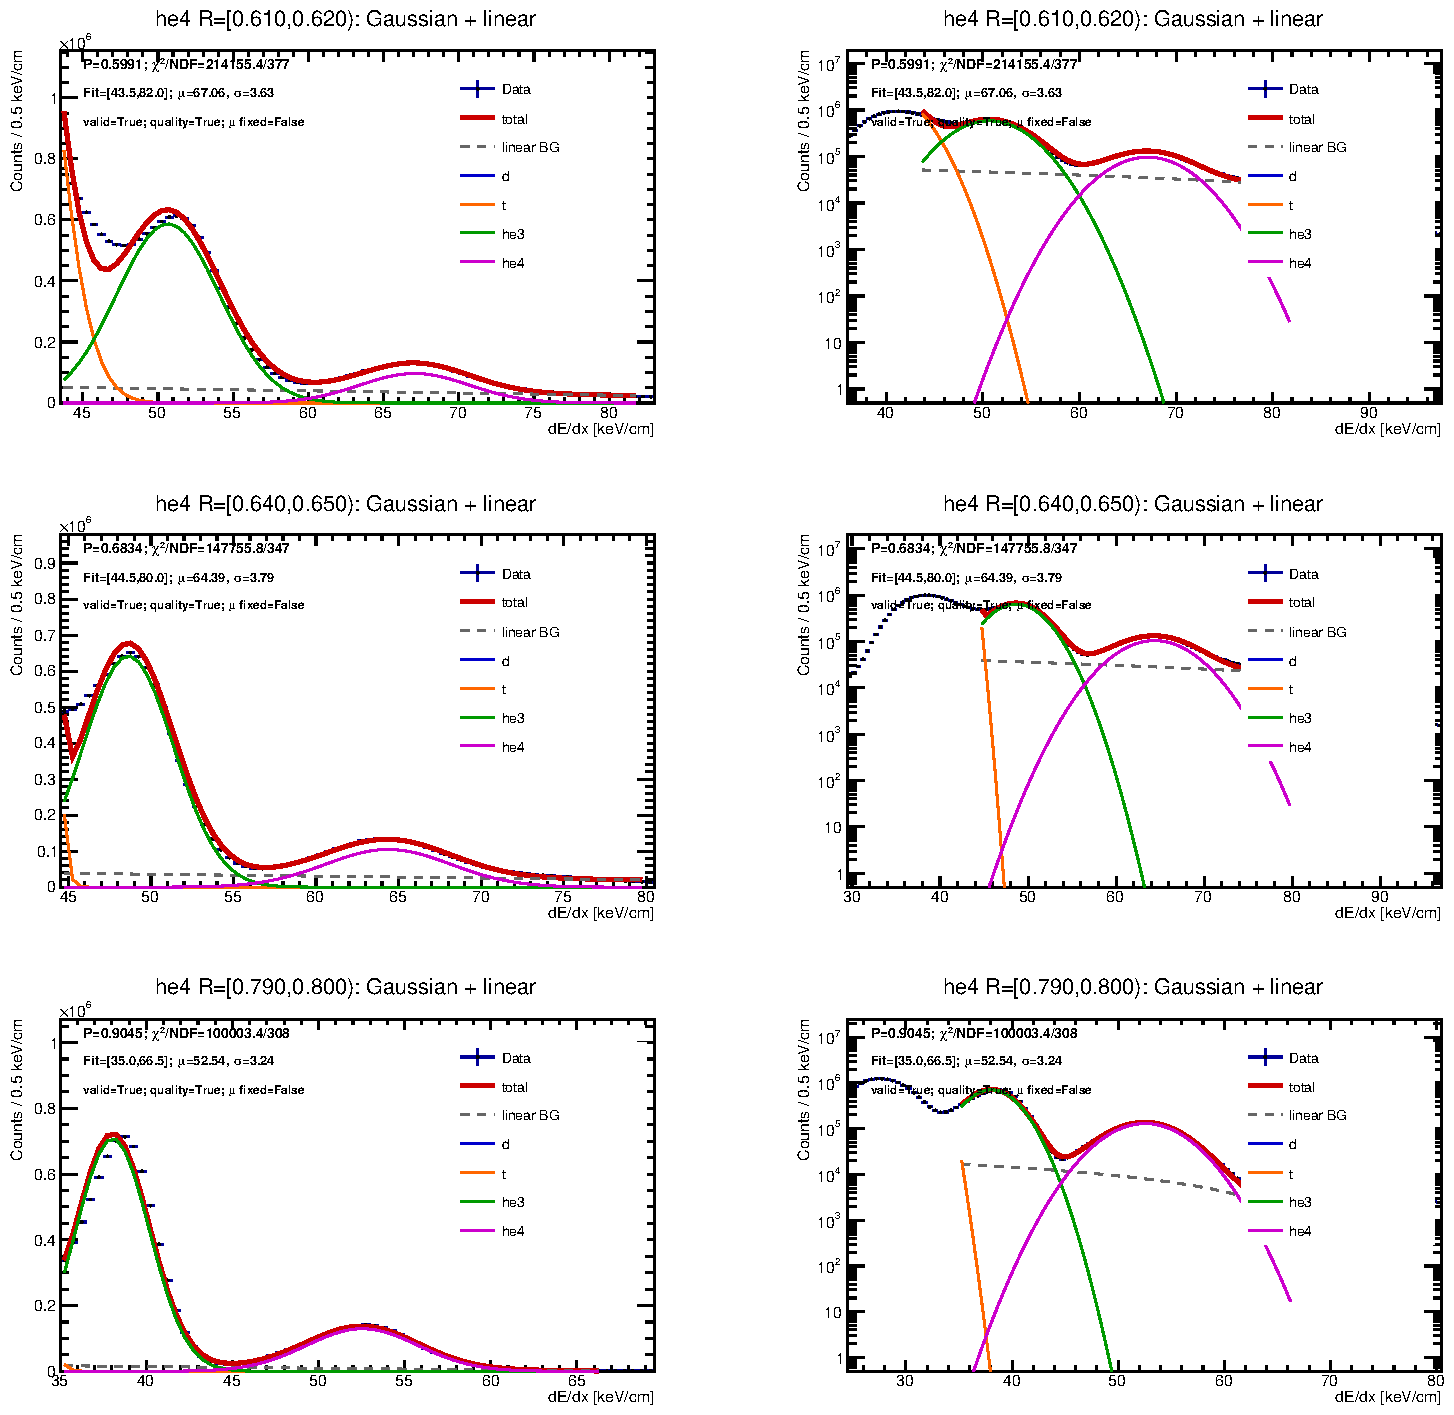
\includegraphics[width=\linewidth,height=.68\textheight,keepaspectratio]{fit_representative_low_linear_01_trim.png}\end{center}
\hspace{0pt}{\jpfont 図}\hspace{0pt}4\hspace{0pt}{\jpfont 　黒：生データ、赤：全モデル、灰破線：}\hspace{0pt}linear\hspace{0pt}{\jpfont 背景（ある領域のみ）、色線：核種成分。}\hspace{0pt}χ²/\allowbreak{}NDF\hspace{0pt}{\jpfont 、}\hspace{0pt}Purity\hspace{0pt}{\jpfont 、}\hspace{0pt}fit\hspace{0pt}{\jpfont 範囲、中心・幅、数値成立と支持フラグを表示。予測曲線は}\hspace{0pt}fit\hspace{0pt}{\jpfont 範囲内のみ描画した。}\hspace{0pt}

\hspace{0pt}{\jpfont 低}\hspace{0pt}R\hspace{0pt}{\jpfont では}\hspace{0pt}fit\hspace{0pt}{\jpfont 後の}\hspace{0pt}³He\hspace{0pt}{\jpfont 低側半値を全}\hspace{0pt}GL3\hspace{0pt}{\jpfont 点で含む。右の}\hspace{0pt}log\hspace{0pt}{\jpfont は縦軸表示で、}\hspace{0pt}lognormal\hspace{0pt}{\jpfont 応答を用いたものではない。}\hspace{0pt}


\clearpage
\section*{6. \hspace{0pt}{\jpfont 代表}\hspace{0pt}fit\hspace{0pt}{\jpfont ：中}\hspace{0pt}R Gaussian\hspace{0pt}{\jpfont のみ}\hspace{0pt}}
R=[0.80,0.81)\hspace{0pt}{\jpfont 、}\hspace{0pt}[1.20,1.21)\hspace{0pt}{\jpfont 、}\hspace{0pt}[1.60,1.61) GeV/\allowbreak{}c\hspace{0pt}{\jpfont 。各段で左}\hspace{0pt}linear\hspace{0pt}{\jpfont 、右}\hspace{0pt}log\hspace{0pt}{\jpfont 表示。}\hspace{0pt}smooth\hspace{0pt}{\jpfont 背景を完全に除く。}\hspace{0pt}Gaussian\hspace{0pt}{\jpfont は他核種の混入も含む}\hspace{0pt}4\hspace{0pt}{\jpfont 成分であり、}\hspace{0pt}⁴He\hspace{0pt}{\jpfont 信号だけの}\hspace{0pt}fit\hspace{0pt}{\jpfont ではない。}\hspace{0pt}

\begin{center}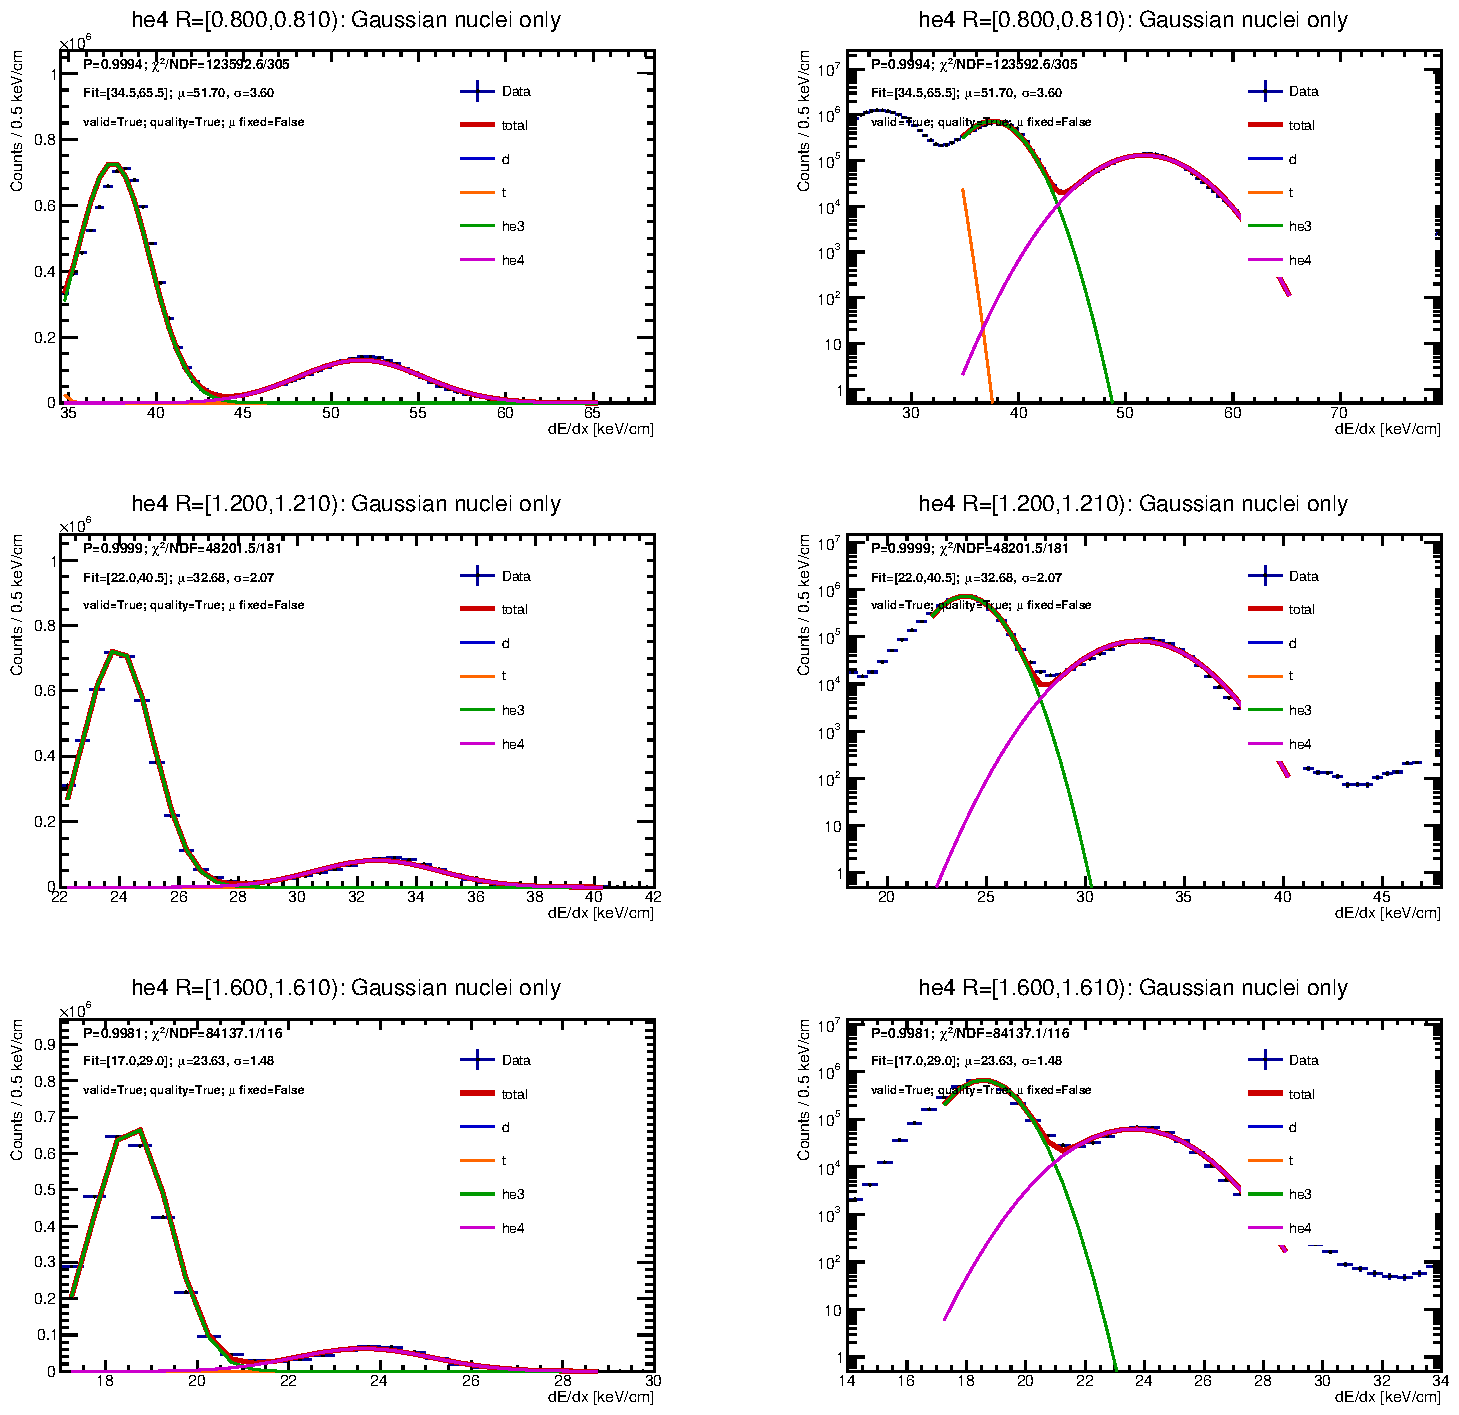
\includegraphics[width=\linewidth,height=.68\textheight,keepaspectratio]{fit_representative_low_none_01_trim.png}\end{center}
\hspace{0pt}{\jpfont 図}\hspace{0pt}5\hspace{0pt}{\jpfont 　黒：生データ、赤：全モデル、灰破線：}\hspace{0pt}linear\hspace{0pt}{\jpfont 背景（ある領域のみ）、色線：核種成分。}\hspace{0pt}χ²/\allowbreak{}NDF\hspace{0pt}{\jpfont 、}\hspace{0pt}Purity\hspace{0pt}{\jpfont 、}\hspace{0pt}fit\hspace{0pt}{\jpfont 範囲、中心・幅、数値成立と支持フラグを表示。予測曲線は}\hspace{0pt}fit\hspace{0pt}{\jpfont 範囲内のみ描画した。}\hspace{0pt}

\hspace{0pt}{\jpfont 低}\hspace{0pt}R\hspace{0pt}{\jpfont では}\hspace{0pt}fit\hspace{0pt}{\jpfont 後の}\hspace{0pt}³He\hspace{0pt}{\jpfont 低側半値を全}\hspace{0pt}GL3\hspace{0pt}{\jpfont 点で含む。右の}\hspace{0pt}log\hspace{0pt}{\jpfont は縦軸表示で、}\hspace{0pt}lognormal\hspace{0pt}{\jpfont 応答を用いたものではない。}\hspace{0pt}


\clearpage
\section*{7. \hspace{0pt}{\jpfont 代表}\hspace{0pt}fit\hspace{0pt}{\jpfont ：高}\hspace{0pt}R ⁠⁴He Gaussian\hspace{0pt}{\jpfont ＋}\hspace{0pt}linear\hspace{0pt}{\jpfont のみ}\hspace{0pt}}
R=[2.00,2.05)\hspace{0pt}{\jpfont 、}\hspace{0pt}[2.20,2.25)\hspace{0pt}{\jpfont 、}\hspace{0pt}[3.00,3.05) GeV/\allowbreak{}c\hspace{0pt}{\jpfont 。各段で左}\hspace{0pt}linear\hspace{0pt}{\jpfont 、右}\hspace{0pt}log\hspace{0pt}{\jpfont 表示。}\hspace{0pt}TOF\hspace{0pt}{\jpfont は}\hspace{0pt}d\hspace{0pt}{\jpfont と同じ}\hspace{0pt}m²\hspace{0pt}{\jpfont 窓。}\hspace{0pt}fit\hspace{0pt}{\jpfont は}\hspace{0pt}⁴He\hspace{0pt}{\jpfont と}\hspace{0pt}linear\hspace{0pt}{\jpfont 背景だけで、}\hspace{0pt}d/\allowbreak{}t/\allowbreak{}³He\hspace{0pt}{\jpfont の寄与は}\hspace{0pt}0\hspace{0pt}{\jpfont 、自由パラメータにも含めない。}\hspace{0pt}

\begin{center}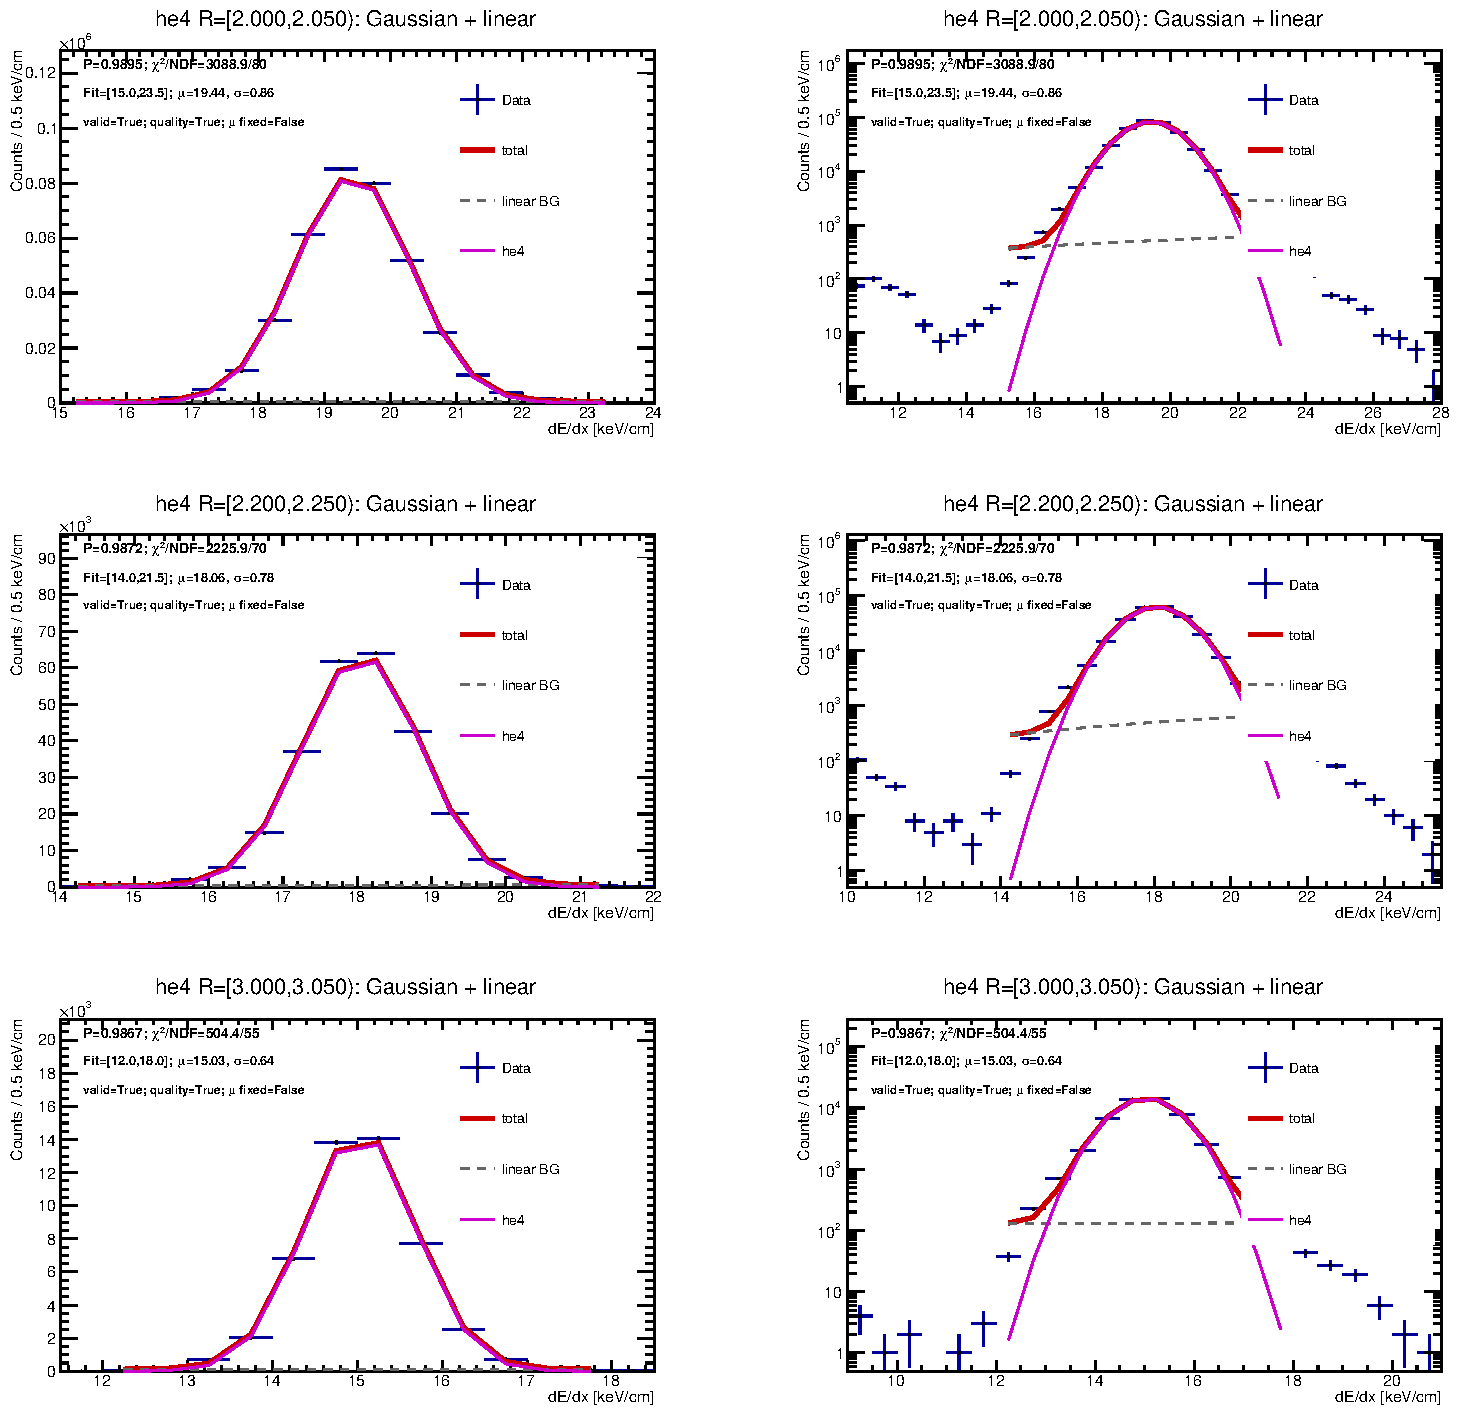
\includegraphics[width=\linewidth,height=.68\textheight,keepaspectratio]{fit_representative_high_linear_01_trim.png}\end{center}
\hspace{0pt}{\jpfont 図}\hspace{0pt}6\hspace{0pt}{\jpfont 　黒：生データ、赤：全モデル、灰破線：}\hspace{0pt}linear\hspace{0pt}{\jpfont 背景（ある領域のみ）、色線：核種成分。}\hspace{0pt}χ²/\allowbreak{}NDF\hspace{0pt}{\jpfont 、}\hspace{0pt}Purity\hspace{0pt}{\jpfont 、}\hspace{0pt}fit\hspace{0pt}{\jpfont 範囲、中心・幅、数値成立と支持フラグを表示。予測曲線は}\hspace{0pt}fit\hspace{0pt}{\jpfont 範囲内のみ描画した。}\hspace{0pt}

\hspace{0pt}{\jpfont 高}\hspace{0pt}R\hspace{0pt}{\jpfont は他核種込みの旧}\hspace{0pt}fit\hspace{0pt}{\jpfont を再利用せず、新しいモデルで}\hspace{0pt}60\hspace{0pt}{\jpfont 区間を全て再}\hspace{0pt}fit\hspace{0pt}{\jpfont した。非表示で隠しただけの核種成分はない。}\hspace{0pt}


\clearpage
\section*{8. \hspace{0pt}{\jpfont 低}\hspace{0pt}R Purity\hspace{0pt}{\jpfont と評価可能域}\hspace{0pt}}
\begin{center}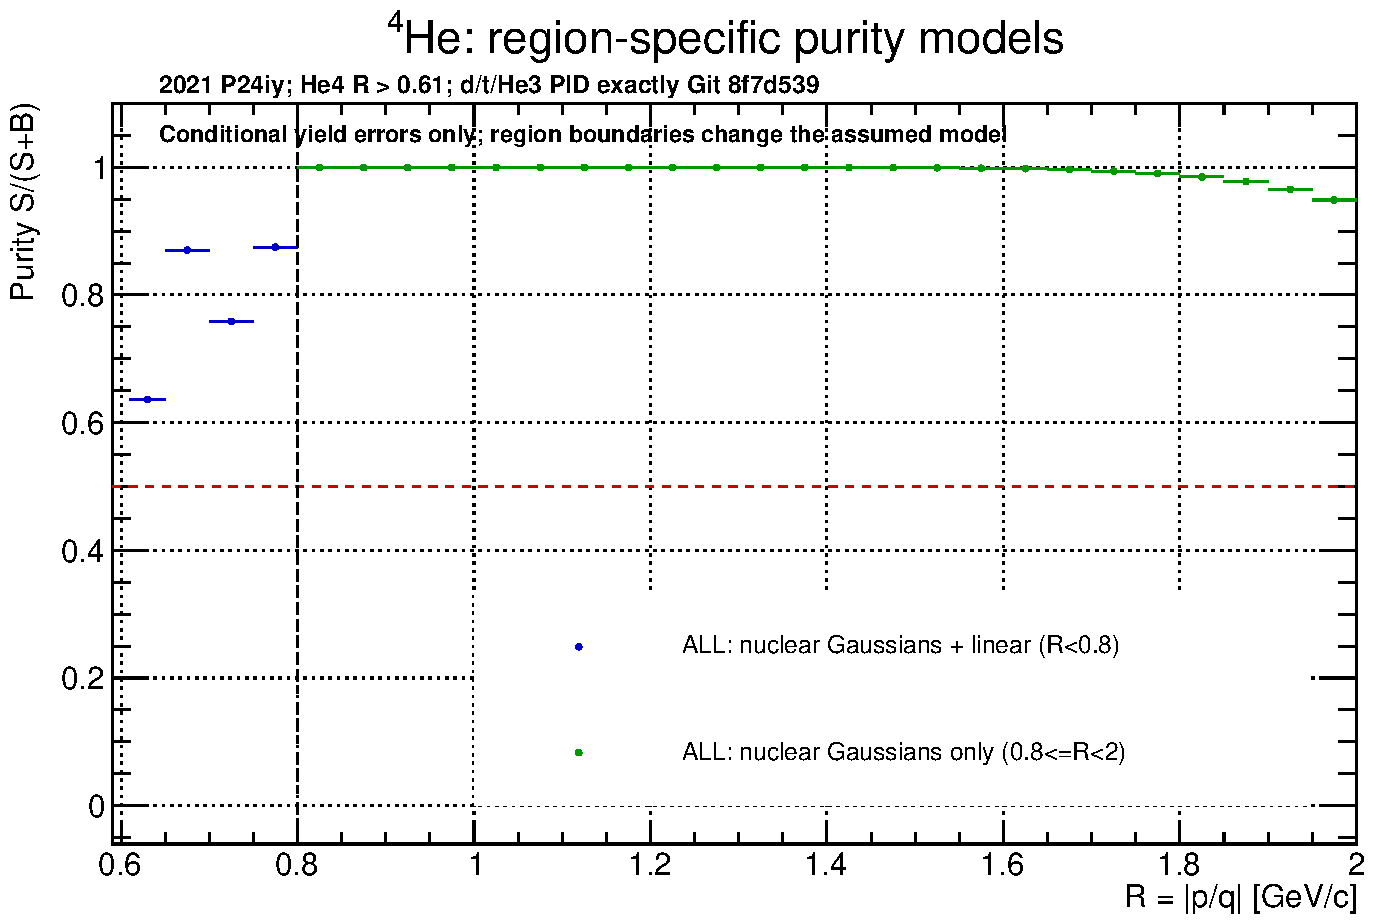
\includegraphics[width=\linewidth,height=.57\textheight,keepaspectratio]{purity_vs_p_over_q_02_trim.png}\end{center}
\hspace{0pt}{\jpfont 図}\hspace{0pt}7\hspace{0pt}{\jpfont 　低}\hspace{0pt}R\hspace{0pt}{\jpfont 表示。}\hspace{0pt}0.80\hspace{0pt}{\jpfont で}\hspace{0pt}smooth\hspace{0pt}{\jpfont 背景の仮定が変わるため、}\hspace{0pt}Purity\hspace{0pt}{\jpfont の段差を同一モデルでの連続改善と解釈しない。}\hspace{0pt}

\begin{center}\small\begin{tabular}{lrr}\toprule
\hspace{0pt}{\jpfont 領域}\hspace{0pt} & \hspace{0pt}{\jpfont 支持}\hspace{0pt}/\allowbreak{}\hspace{0pt}{\jpfont 全区間}\hspace{0pt} & \hspace{0pt}{\jpfont 支持点の最小}\hspace{0pt}Purity\\\midrule
{}ALL\hspace{0pt}{\jpfont ＋}\hspace{0pt}linear & 4/\allowbreak{}4 & 63.66\%\\
{}ALL\hspace{0pt}{\jpfont 背景なし}\hspace{0pt} & 24/\allowbreak{}24 & 94.88\%\\
{}TOF ⁠⁴He\hspace{0pt}{\jpfont ＋}\hspace{0pt}linear & 48/\allowbreak{}60 & 98.06\%\\\bottomrule\end{tabular}\end{center}
\hspace{0pt}{\jpfont 低}\hspace{0pt}R28\hspace{0pt}{\jpfont 区間は全て支持条件を通過。高}\hspace{0pt}R\hspace{0pt}{\jpfont 支持点の範囲は}\hspace{0pt}R=2.00–4.45\hspace{0pt}{\jpfont で、}\hspace{0pt}4.30–4.35\hspace{0pt}{\jpfont に未支持の穴がある。}\hspace{0pt}4.45\hspace{0pt}{\jpfont 以上も未支持であり、穴をつなぐ外挿・追加}\hspace{0pt}veto\hspace{0pt}{\jpfont ・単一上限は設定しない。}\hspace{0pt}


\clearpage
\section*{9. \hspace{0pt}{\jpfont 品質、誤差と再現性}\hspace{0pt}}
\hspace{0pt}{\jpfont 支持フラグは従来の数値成立、形状誤差、}\hspace{0pt}identity\hspace{0pt}{\jpfont 、選択領域内残差等の条件で決まる。支持されたことは}\hspace{0pt}χ²/\allowbreak{}NDF≈1\hspace{0pt}{\jpfont やモデルの物理的正しさを保証しない。未支持の全}\hspace{0pt}12\hspace{0pt}{\jpfont 区間も}\hspace{0pt}fit\hspace{0pt}{\jpfont 集に掲載する。}\hspace{0pt}

\begin{center}\small\begin{tabular}{lr}\toprule
\hspace{0pt}{\jpfont 未支持}\hspace{0pt}R\hspace{0pt}{\jpfont 区間}\hspace{0pt} & \hspace{0pt}{\jpfont 主な原因}\hspace{0pt}\\\midrule
{}4.30–4.35 & \hspace{0pt}{\jpfont 局所残差}\hspace{0pt}\\
{}4.45–4.50 & \hspace{0pt}{\jpfont 局所残差}\hspace{0pt}\\
{}4.50–4.55 & \hspace{0pt}{\jpfont 局所残差}\hspace{0pt}\\
{}4.55–4.60 & \hspace{0pt}{\jpfont 局所残差・形状支持}\hspace{0pt}\\
{}4.60–4.65 & \hspace{0pt}{\jpfont 局所残差}\hspace{0pt}\\
{}4.65–4.70 & \hspace{0pt}{\jpfont 局所残差・形状支持}\hspace{0pt}\\
{}4.70–4.75 & \hspace{0pt}{\jpfont 局所残差}\hspace{0pt}\\
{}4.75–4.80 & \hspace{0pt}{\jpfont 局所残差}\hspace{0pt}\\
{}4.80–4.85 & \hspace{0pt}{\jpfont 局所残差・形状支持}\hspace{0pt}\\
{}4.85–4.90 & \hspace{0pt}{\jpfont 局所残差・形状支持}\hspace{0pt}\\
{}4.90–4.95 & \hspace{0pt}{\jpfont 局所残差・形状支持}\hspace{0pt}\\
{}4.95–5.00 & \hspace{0pt}{\jpfont 局所残差・形状支持}\hspace{0pt}\\\bottomrule\end{tabular}\end{center}
\hspace{0pt}{\jpfont 誤差はモデル・形状を条件とした収量誤差。集約では分母で重み付けして線形和をとる保守的な上限であり、応答形状・較正位置・背景選択・高}\hspace{0pt}R\hspace{0pt}{\jpfont で除いた他核種の完全な系統誤差ではない。背景なしで}\hspace{0pt}Purity\hspace{0pt}{\jpfont が}\hspace{0pt}1\hspace{0pt}{\jpfont 近くなる点も仮定の影響を含む。}\hspace{0pt}

\hspace{0pt}{\jpfont 検証：}\hspace{0pt}d/\allowbreak{}t/\allowbreak{}³He\hspace{0pt}{\jpfont の}\hspace{0pt}Git\hspace{0pt}{\jpfont 一致、元ヒスト不変、中}\hspace{0pt}R\hspace{0pt}{\jpfont 背景}\hspace{0pt}=0\hspace{0pt}{\jpfont 、高}\hspace{0pt}R d/\allowbreak{}t/\allowbreak{}³He\hspace{0pt}{\jpfont 成分}\hspace{0pt}=0\hspace{0pt}{\jpfont を確認。}\hspace{0pt}556\hspace{0pt}{\jpfont 件の独立生計数、}\hspace{0pt}417\hspace{0pt}{\jpfont 点の}\hspace{0pt}³He\hspace{0pt}{\jpfont 半値包含、}\hspace{0pt}199\hspace{0pt}{\jpfont 件の基準}\hspace{0pt}/\allowbreak{}\hspace{0pt}{\jpfont 候補の}\hspace{0pt}likelihood\hspace{0pt}{\jpfont 一致を確認した。旧入力}\hspace{0pt}SHA\hspace{0pt}{\jpfont と全}\hspace{0pt}PDF\hspace{0pt}{\jpfont の読戻しを検証し、}\hspace{0pt}completed.json\hspace{0pt}{\jpfont に保存する。}\hspace{0pt}

\hspace{0pt}{\jpfont 再現ツール：}\hspace{0pt}tools/\allowbreak{}nuclear\_\allowbreak{}pid\_\allowbreak{}he4\_\allowbreak{}20261022/\allowbreak{}\hspace{0pt}{\jpfont 。}\hspace{0pt}

\hspace{0pt}{\jpfont 設定・係数・選択条件・集約値・各}\hspace{0pt}native\hspace{0pt}{\jpfont 区間の値、ソースとコマンドを同梱。}\hspace{0pt}Git\hspace{0pt}{\jpfont 元ヘッダと候補差分も保存。}\hspace{0pt}

mainconf\hspace{0pt}{\jpfont ：}\hspace{0pt}main\_\allowbreak{}auau3p85\_\allowbreak{}anaFemtoLambda\_\allowbreak{}4He\_\allowbreak{}KFParticle.yaml\hspace{0pt}{\jpfont 。}\hspace{0pt}STAR SL24y/\allowbreak{}ROOT5\hspace{0pt}{\jpfont の既存}\hspace{0pt}wrapper\hspace{0pt}{\jpfont で実行。}\hspace{0pt}2021 P24iy\hspace{0pt}{\jpfont キャッシュのローカル}\hspace{0pt}study\hspace{0pt}{\jpfont で新規}\hspace{0pt}jobid/\allowbreak{}configlog\hspace{0pt}{\jpfont なし。本番}\hspace{0pt}PID\hspace{0pt}{\jpfont 反映・}\hspace{0pt}job\hspace{0pt}{\jpfont 投入・}\hspace{0pt}hadd\hspace{0pt}{\jpfont ・}\hspace{0pt}commit/\allowbreak{}push\hspace{0pt}{\jpfont なし。}\hspace{0pt}


\end{document}
